\documentclass{BeamerTemplate}
\title{Module 1 - Introduction aux probabilités}
\subtitle{STT-1000 Probabilités et statistique}
\date{\today}

% Lien discret vers la page de réponses, ajouté au pied de page à côté du numéro
% (ne prend aucune place sur la diapo). Usage, n'importe où dans la diapo : \lienreponse{rep-ex1}
\newcommand{\cibleReponse}{}
\newcommand{\lienreponse}[1]{\gdef\cibleReponse{#1}}
\addtobeamertemplate{footline}{}{%
  \ifx\cibleReponse\empty\else
    \begin{tikzpicture}[remember picture,overlay]
      \node[anchor=south east, inner sep=0pt] at ([xshift=-1.5cm,yshift=0.2cm]current page.south east)
        {\hyperlink{\cibleReponse}{\scriptsize\color{gray}Réponse~$\rightarrow$}};
    \end{tikzpicture}%
    \global\let\cibleReponse\empty
  \fi}
% Lien de retour vers l'exemple, dans les pages de réponses
\newcommand{\retour}[2]{\hyperlink{#1}{\textbf{#2}~{\color{gray}$\hookleftarrow$}}}

\begin{document}
\begin{frame}[t]
  \titlepage
\end{frame}

\section{Importance de la statistique}

\begin{frame}{Importance de la statistique}
  \begin{Boite}{Pourquoi un cours de statistique?}
    Pour concevoir ou analyser des systèmes et des phénomènes aléatoires, c'est-à-dire non déterministes.
  \end{Boite}
  Exemples :
  \begin{itemize}
    \item fiabilité des disques durs d'un centre de données;
    \item temps de réponse d'un site web aux heures de pointe;
    \item demande en électricité d'un grand complexe de serveurs;
    \item taux d'erreur d'un modèle d'apprentissage automatique sur de nouvelles données.
  \end{itemize}
\end{frame}

\begin{frame}{Probabilités ou statistique?}
  \small
  \begin{Boite}{Probabilités}
    Outil mathématique formel qui sert à décrire et à modéliser les comportements aléatoires.
  \end{Boite}
  On connaît les \enquote{paramètres} du phénomène; on décrit ce qu'on peut en attendre.\\
  Exemple : on lance un dé équilibré à 6 faces. Quelle est la probabilité d'obtenir un 3?

  \pause

  \begin{Boite}{Statistique}
    Étude quantitative des caractéristiques d'une \enquote{population} à partir d'observations.
  \end{Boite}
  On ne connaît pas les \enquote{paramètres} du phénomène : c'est ce qu'on cherche à estimer.\\
  Exemple : le dé virtuel d'un jeu vidéo est-il vraiment équilibré?

  \pause

  Comprendre les probabilités et la statistique est indispensable pour prendre des décisions en situation d'incertitude.
\end{frame}

\section{Expérience aléatoire}

\begin{frame}{Expérience aléatoire et espace échantillonnal}
\begin{Boite}{Expérience aléatoire $\mathcal{E}$}
    Expérience dont le résultat dépend du hasard et ne peut donc pas être prédit avec certitude.
\end{Boite}

\begin{Boite}{Espace échantillonnal $\mathcal{U}$}
    Ensemble de tous les résultats possibles de l'expérience $\mathcal{E}$.
\end{Boite}

\begin{itemize}
\item $\mathcal{U}$ est \alerter{discret} s'il est fini ou dénombrable\\
(ex. : l'ensemble des entiers);
\item $\mathcal{U}$ est \alerter{continu} s'il est non dénombrable\\
(ex. : un intervalle de la droite réelle).
\end{itemize}

\end{frame}


\begin{frame}{Espace échantillonnal : exemples}
Quel est l'espace échantillonnal de chacune de ces expériences?

\begin{itemize}
    \item $\mathcal{E}_1$ : on lance un dé et on note le chiffre obtenu;
    \vspace{1cm}
    \item $\mathcal{E}_2$ : on pige une carte parmi les quatre rois d'un jeu de cartes standard;
    \vspace{1cm}
    \item $\mathcal{E}_3$ : on compte le nombre de requêtes reçues par un serveur web en une heure;
    \vspace{1cm}
    \item $\mathcal{E}_4$ : on mesure le temps de réponse (en ms) d'un site web à une requête.
    \vspace{1cm}
\end{itemize}
\end{frame}

\begin{frame}{Événements}
\begin{Boite}{Événement}
    Sous-ensemble de l'espace échantillonnal $\mathcal{U}$. On le désigne par une lettre majuscule.
\end{Boite}
Retour aux expériences précédentes :
\begin{itemize}
    \item $\mathcal{E}_1$ : $A=$ \enquote{le dé indique un nombre pair} $=\{2,4,6\}$
    \item $\mathcal{E}_2$ : $B=$ \enquote{on pige un roi noir} $=\{R\spadesuit,R\clubsuit\}$
    \item $\mathcal{E}_3$ : $C=$ \enquote{le serveur reçoit moins de 100 requêtes} $=\{0,1,2,\ldots,99\}$
    \item $\mathcal{E}_4$ : $D=$ \enquote{le temps de réponse dépasse 150 ms} $=(150,\infty)$
\end{itemize}

\end{frame}


\begin{frame}{Opérations sur les événements}
\begin{tabular}{lll}
1) Complément de $A$ : $\overline{A}$&\hspace{1cm}&2) Inclusion de $B$ dans $A$ : $B \subset A $\\
&&\\
\begin{tabular}{|ccc|}\hline
&&\\[-0.2cm]
\hspace{0.05cm}&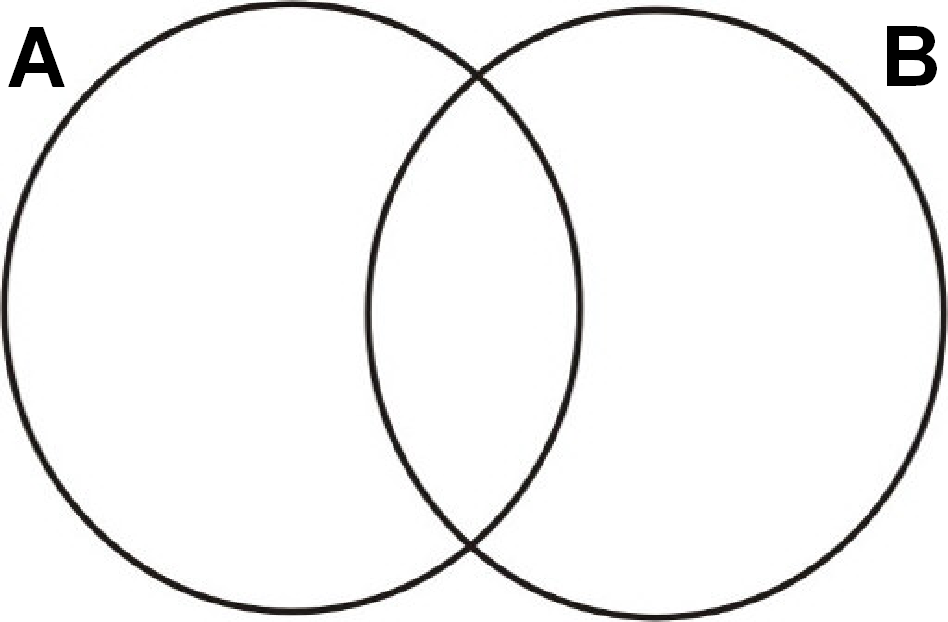
\includegraphics[width=2.7cm]{venn.pdf}&\hspace{.05cm}\\
\hline
\end{tabular}&&
\begin{tabular}{|ccc|}\hline
&&\\[-0.2cm]
\hspace{0.05cm}& \hspace{2.7cm} &\hspace{.05cm}\\[1cm]&&\\
\hline
\end{tabular}\\

&&\\
3) Intersection de $A$ et $B$ : $A\cap B$&\hspace{1cm}& 4) Union de $A$ et $B$ : $A\cup B$\\&&\\
\begin{tabular}{|ccc|}\hline
&&\\[-0.2cm]
\hspace{0.05cm}&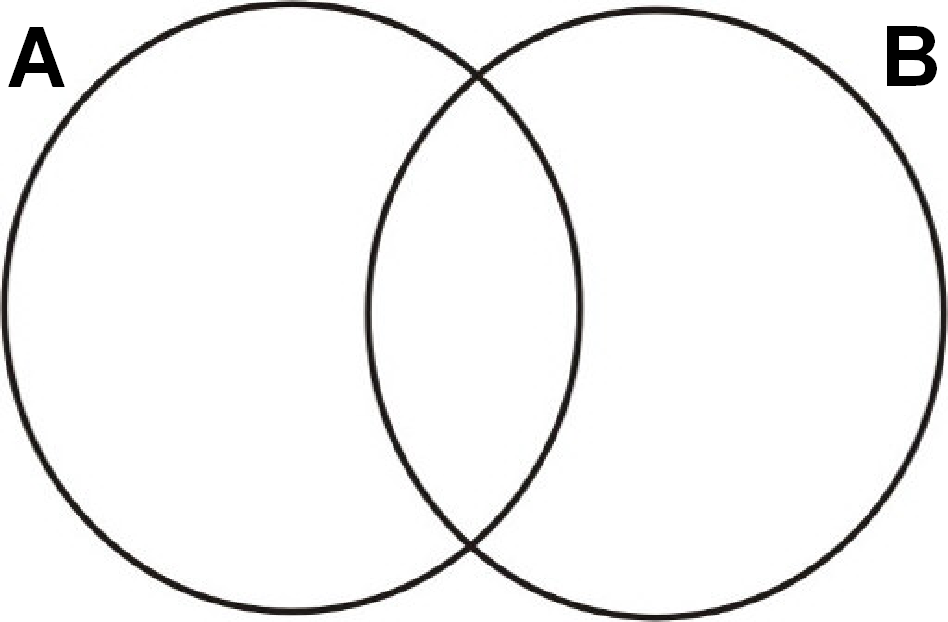
\includegraphics[width=2.7cm]{venn.pdf}&\hspace{.05cm}\\
\hline
\end{tabular}
&\hspace{1cm}&
\begin{tabular}{|ccc|}\hline
&&\\[-0.2cm]
\hspace{0.05cm}&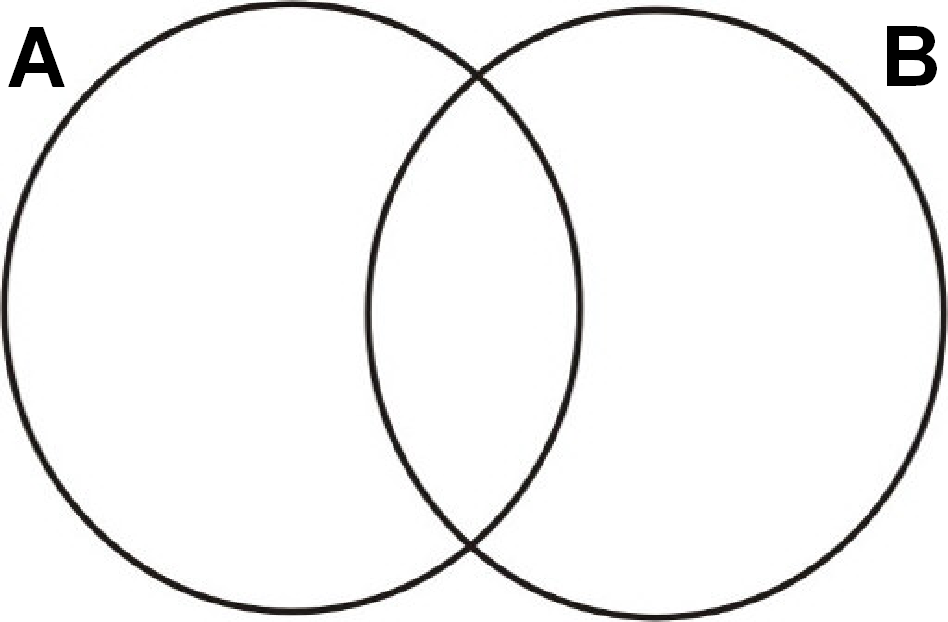
\includegraphics[width=2.7cm]{venn.pdf}&\hspace{.05cm}\\
\hline
\end{tabular}
\end{tabular}

\vspace{1cm}
\end{frame}

\begin{frame}[t]{Ensemble vide, inclusion et égalité}
\begin{itemize}
    \item L'\alerter{ensemble vide}, noté $\emptyset$, ne contient aucun élément.
    \item $\emptyset$ est inclus dans tout ensemble : $\emptyset \subset A$, $\forall A$.
    \item Tout événement est inclus dans $\mathcal{U}$ : $A\subset \mathcal{U}$, $\forall A$.
    \item Deux ensembles $A$ et $B$ sont \alerter{égaux} si et seulement si chacun est inclus dans l'autre :\\
    $A=B \iff A\subset B$ et $B\subset A$.
    \item L'inclusion est transitive : si $A\subset B$ et $B\subset C$, alors $A\subset C$.
    \item L'ordre des éléments d'un ensemble n'a pas d'importance :\\
    $\{1,2,3,4,5,6\}=\{6,5,4,3,2,1\}$.
\end{itemize}
\end{frame}

\begin{frame}[t]{Lois de l'algèbre des ensembles}
\small
\begin{columns}[T]
\begin{column}{0.48\textwidth}
    Lois d'identité
    \begin{align*}
        A\cup \emptyset &= A & A\cup \mathcal{U} &= \mathcal{U}\\
        A\cap \emptyset &= \emptyset & A\cap \mathcal{U} &= A
    \end{align*}
    Lois de De Morgan
    \begin{align*}
        \overline{A\cup B}&=\overline{A}\cap \overline{B}\\
        \overline{A\cap B}&=\overline{A}\cup \overline{B}
    \end{align*}
\end{column}
\begin{column}{0.48\textwidth}
    Lois associatives
    \begin{align*}
        A\cup (B\cup C) &= (A\cup B)\cup C\\
        A\cap (B\cap C) &= (A\cap B)\cap C
    \end{align*}
    Lois distributives
    \begin{align*}
        A\cup (B\cap C) &= (A\cup B)\cap (A \cup C)\\
        A\cap (B\cup C) &= (A\cap B)\cup (A \cap C)
    \end{align*}
\end{column}
\end{columns}
\end{frame}

\begin{frame}{Événements mutuellement exclusifs}
 \begin{Boite}{Événements mutuellement exclusifs (ou disjoints)}
  Des événements sont \alerter{mutuellement exclusifs} si toutes leurs
  intersections possibles sont vides, c'est-à-dire si \textbf{au plus un}
  de ces événements peut se produire à la fois.
 \end{Boite}

 \medskip

\pause


 Par exemple, $A$, $B$ et $C$ sont mutuellement exclusifs si

  \begin{itemize}
   \item $A\cap B=\emptyset$,
   \item $A\cap C=\emptyset$,
   \item $B\cap C=\emptyset$ et
   \item $A\cap B\cap C=\emptyset$.
 \end{itemize}

\end{frame}

\begin{frame}[t,label=ex1]{Exemple 1}

\centerline{\LARGE\bfseries\alert{QUIZ !}}
 Les événements suivants sont-ils mutuellement exclusifs?
 \medskip

 {\small
  \begin{itemize}\itemsep1.3cm
   \item $\mathcal{E}_1$ : on lance un dé.\\
   $A=$ \enquote{obtenir un nombre pair}, $B=\{5\}$ et $C=\{1\}$.
   \item $\mathcal{E}_4$ : on mesure le temps de réponse d'un site web.\\
   $A=$ \enquote{la réponse prend plus de 150 ms},\\
   $B=$ \enquote{la réponse prend moins de 175 ms} et\\
   $C=$ \enquote{la réponse prend entre 200 et 300 ms}.
   \vspace{1.3cm}
 \end{itemize}
 }
\lienreponse{rep-quiz}
\end{frame}


\section{Probabilités}

\subsection{Définitions et notation}

\begin{frame}[t]

\begin{defn}{}
  Soit une expérience aléatoire $\mathcal{E}$ et son espace échantillonnal
  $\mathcal{U}$. La \alerter{probabilité d'un événement $A$} de $\mathcal{U}$,
  notée \alerter{$P(A)$}, est un nombre réel qui respecte les axiomes suivants :
  \begin{enumerate}
   \item $0\le P(A)\le 1$;
   \item $P(\mathcal{U})=1$;
   \item pour toute suite d'événements \alerter{mutuellement exclusifs}
   $A_1,A_2,\ldots,A_k$ de $\mathcal{U}$,
   $$P(A_1\cup A_2\cup \cdots \cup A_k)=P(A_1)+P(A_2)+\cdots+P(A_k);$$
   \item l'axiome 3 reste vrai quand $k\to\infty$ :\ $P\left(\bigcup_{i=1}\limits^\infty A_i\right)=\sum\limits_{i=1}^\infty P(A_i)$.
  \end{enumerate}
 \end{defn}

\end{frame}

\subsection{Propriétés}

\begin{frame}[t]{Résultats découlant des axiomes}
Les résultats suivants découlent directement des 4 axiomes.
 \begin{itemize}
  \item<1->{\bf Théorème 1.1} : $P(\emptyset)=0$

  {\color{gray}{[$\mathcal{U}$ et $\emptyset$ sont mutuellement
  exclusifs, $\mathcal{U}\cup\emptyset=\mathcal{U}$ et $P(\mathcal{U})=1$...]}}
  \item<2->{\bf Théorème 1.2} : $P(\overline{A})=1-P(A)$

  {\color{gray}{[$A$ et $\overline{A}$ sont mutuellement
  exclusifs et $A\cup\overline{A}=\mathcal{U}$...]}}
  \item<3->{\bf Théorème 1.3} : $P(A\cup B)=P(A)+P(B)-P(A\cap B)$

  \item<4->{\bf Théorème 1.4} :
  $$\begin{array}{lll}
  P(A\cup B\cup C)&=&P(A)+P(B)+P(C)\\&&-P(A\cap B)
   -P(A\cap C)-P(B\cap C)\\&&+P(A\cap B\cap C)\end{array}$$

 \end{itemize}
\end{frame}


\begin{frame}[t,label=ex2]{Exemple 2}

\centerline{\LARGE\bfseries\alert{QUIZ !}}
\begin{minipage}{8cm}{
\small
Vous achetez un nouveau téléphone.\\
On définit les événements suivants :\\
$A$ : \enquote{la carte SIM est défectueuse};\\
$B$ : \enquote{la batterie a une autonomie insuffisante}.\\
}
\end{minipage}

\vspace{.3cm}

Chez ce fournisseur, $P(A)=0{,}05$, $P(B)=0{,}20$ et $P(A \cup B)=0{,}23$.

\begin{enumerate}[{a)}]\itemsep1cm
  \item Quelle est la probabilité que la batterie de votre téléphone ait une autonomie suffisante?
  \item Quelle est la probabilité que votre téléphone présente les deux problèmes?
\end{enumerate}
\lienreponse{rep-quiz}
\end{frame}



\begin{frame}[t,label=ex2s]{Exemple 2 (suite)}
Dans l'exemple précédent, quelle est la probabilité que votre téléphone ne présente aucun des deux problèmes?

 \bigskip

 (Indice : tracez le diagramme de Venn de ces événements et inscrivez les probabilités dans chacune des régions.)

 \bigskip
Rappel : $P(A)=0{,}05$, $P(B)=0{,}20$ et $P(A \cup B)=0{,}23$.
\vspace{3cm}

\lienreponse{rep-ex1}
\end{frame}

\begin{frame}[t,label=ex3]{Exemple 3}

\begin{minipage}{9cm}{
\small
 Dans un programme d'informatique,
 \begin{enumerate}[$\bullet$]
 \item 55\,\% des étudiants utilisent Linux,
 \item 70\,\% des étudiants utilisent un outil d'IA pour coder,
 \item 75\,\% des étudiants sont satisfaits de leur programme.
 \end{enumerate}
 }
 \end{minipage}


 \bigskip
 {\small
 Si on choisit un étudiant au hasard dans ce programme, pouvez-vous déterminer la probabilité qu'il s'agisse...
  \begin{enumerate}[(i)]\itemsep.8cm
 \item d'un étudiant qui n'utilise pas Linux? % 0,45
  \item d'un étudiant qui utilise Linux et qui est satisfait de son programme? % manque d'information
 \end{enumerate}
}
\lienreponse{rep-ex1}
\end{frame}

\begin{frame}[t]{Exemple 3 (suite)}

{\footnotesize
 On vous informe aussi que, dans ce programme,
 \begin{enumerate}[$\bullet$]
 \item 35\,\% des étudiants utilisent Linux et un outil d'IA,
 \item 30\,\% utilisent Linux et un outil d'IA, et sont satisfaits de leur programme,
 \item 5\,\% utilisent Linux, n'utilisent pas d'outil d'IA et sont insatisfaits de leur programme.
 \end{enumerate}
 Pouvez-vous maintenant déterminer la probabilité qu'un étudiant choisi au hasard...
     \begin{enumerate}\itemsep 4mm
      \item[(iii)] utilise Linux et soit satisfait de son programme? % 0,45
      \item[(iv)] n'utilise pas Linux et soit satisfait de son programme? % 0,30
      \item[(v)] n'utilise pas Linux, soit satisfait de son programme et utilise un outil d'IA? % manque d'information
      \item[(vi)] soit satisfait de son programme ou utilise Linux? % 0,85
     \end{enumerate}
}
\lienreponse{rep-ex1}
\end{frame}

\begin{frame}[t]{Exemple 3 : piste de solution}

{\small
 Remplissez toutes les zones mutuellement exclusives d'un diagramme de Venn, où
 $L=$ \enquote{l'étudiant utilise Linux}, $I=$ \enquote{l'étudiant utilise un outil d'IA}
 et $S=$ \enquote{l'étudiant est satisfait de son programme}.

 \medskip
 Rappel des données : $P(L)=0{,}55$; $P(I)=0{,}70$; $P(S)=0{,}75$; $P(L\cap I)=0{,}35$; $P(L\cap I\cap S)=0{,}30$; $P(L\cap \overline{I}\cap \overline{S})=0{,}05$.
}

\begin{center}
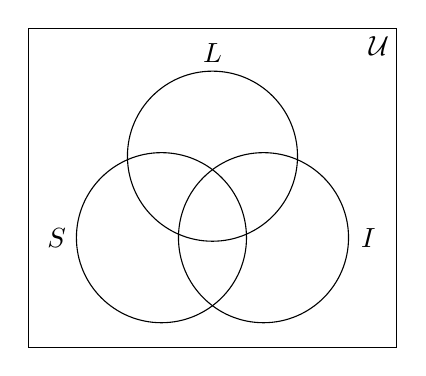
\begin{tikzpicture}[scale=0.9]
  \draw (-2.6,-2.15) rectangle (2.6,2.35);
  \draw (0,0.55) circle (1.2);
  \draw (0.72,-0.6) circle (1.2);
  \draw (-0.72,-0.6) circle (1.2);
  \node at (0,2.0) {$L$};
  \node at (2.2,-0.6) {$I$};
  \node at (-2.2,-0.6) {$S$};
  \node at (2.35,2.1) {$\mathcal{U}$};
\end{tikzpicture}
\end{center}
\end{frame}
\begin{frame}[t]{Exemple 3 : des infos partielles}
\begin{enumerate}
\item[(vii)] Si on vous disait que l'étudiant pigé est satisfait de son programme, pourriez-vous déterminer la probabilité qu'il utilise Linux?

\vspace{1.3cm}

\item[(viii)] Sauriez-vous déduire de ces informations la probabilité qu'un étudiant qui utilise Linux, choisi au hasard, utilise aussi un outil d'IA?

\vspace{1.3cm}
\end{enumerate}

Pour faire ces calculs, il faut tenir compte d'une information partielle, qui réduit l'espace échantillonnal. Ce sont des \textit{probabilités conditionnelles}...

\lienreponse{rep-ex1}
\end{frame}

\section{Probabilités conditionnelles}



\begin{frame}[t]
 \begin{Boite}{Probabilité conditionnelle}
  Soient $A$ et $B$ deux événements de $\mathcal{U}$, avec $P(B)>0$. La
  \alert{probabilité conditionnelle} de $A$ sachant que $B$ s'est réalisé est
  $$P(A|B)=\frac{P(A\cap B)}{P(B)}.$$
 \end{Boite}
\end{frame}

\begin{frame}[t]{Propriétés de la probabilité conditionnelle}
 Une probabilité conditionnelle a toutes les propriétés d'une probabilité :

 \begin{enumerate}\itemsep3mm
  \item $0\le P(A|B)\le 1$;
  \item $P(\mathcal{U}|B)=P(B|B)=1$;
  \item si $A_1,\ldots,A_k$ sont des événements \alerter{mutuellement
  exclusifs}, alors $P\left(\left.\bigcup\limits_{i=1}^kA_i\right|B\right)=\sum\limits_{i=1}^k P(A_i|B)$;
  \item la propriété 3 reste vraie quand $k\to\infty$.
 \end{enumerate}
\end{frame}

\begin{frame}[t]{Règle de multiplication}
La définition de la probabilité conditionnelle permet de trouver $P(A\cap B)$ :
$$P(A|B)=\frac{P(A\cap B)}{P(B)}\quad\Leftrightarrow\quad P(A\cap B)=P(A|B)P(B).$$
On appelle parfois cette formule la \enquote{règle de multiplication}.

\medskip
Elle se généralise à plus de deux événements :
$$P(A\cap B\cap C)=P(A)\,P(B|A)\,P(C|A\cap B),$$
et ainsi de suite pour $k$ événements.
\end{frame}
\begin{frame}[t,label=ex4]{Exemple 4}

{\small
 \begin{enumerate}[$\bullet$]\itemsep3mm
 \item 70\,\% des requêtes reçues par votre application sont traitées par le serveur A; les autres sont traitées par le serveur B.
 \item 25\,\% de toutes les requêtes échouent (délai d'attente dépassé).
 \item 10\,\% de toutes les requêtes sont traitées par le serveur A \emph{et} échouent.
 \item[a)] Une requête a été traitée par le serveur A. Quelle est la probabilité qu'elle ait échoué?
     \end{enumerate}
     }
\lienreponse{rep-ex1}
\end{frame}

\begin{frame}[t]{Exemple 4 (suite)}

{\small
 \begin{enumerate}[$\bullet$]
\item[b)] Une requête a échoué. Quelle est la probabilité qu'elle ait été traitée par le serveur B?
     \end{enumerate}
     }
\lienreponse{rep-ex1}
\end{frame}

\begin{frame}[t,label=quizpab]

\centerline{\LARGE\bfseries\alert{QUIZ !}}
Supposons $P(B)>0$.
\vspace{3mm}

\begin{itemize}\itemsep1.5cm
\item Que vaut $P(A|B)$ si $B\subset A$?

\item Que vaut $P(A|B)$ si $A\subset B$?

\item Que vaut $P(A|B)$ si $A$ et $B$ sont mutuellement exclusifs?
\vspace{1cm}
\end{itemize}
\lienreponse{rep-quiz}
\end{frame}

\subsection{Indépendance}

\begin{frame}[t]{Indépendance de deux événements}

 \bigskip
 Je lance un dé, puis une pièce de monnaie. \\Soient les événements\\
  $A=$ \enquote{le dé indique 6} et \\
  $B=$ \enquote{la pièce tombe sur face}. \\

  \bigskip

Que $A$ se réalise ou non ne change rien à la probabilité que la pièce tombe sur face!
\bigskip

On dit alors que $A$ et $B$ sont \alerter{indépendants}. Voyons une définition mathématique de l'indépendance.
\end{frame}

\begin{frame}[t]
 \begin{Boite}{Indépendance de deux événements}
  Soient $A$ et $B$ deux événements de $\mathcal{U}$. On dit que $A$ et $B$
  sont \alert{indépendants, ce qu'on note $A\perp B$}, si et seulement si
  $$P(A\cap B) = P(A)P(B).$$
 \end{Boite}

    \begin{Boite}{Lien avec les probabilités conditionnelles}
   Supposons que $P(B)>0$, de sorte que $P(A|B)$ est bien définie.\\
   \alert{Si $A$ et $B$ sont indépendants}, alors
   $$P(A|B)=P(A).$$
   Réciproquement, si $P(A|B)=P(A)$, alors $A$ et $B$ sont indépendants.
  \end{Boite}
\end{frame}

\begin{frame}[t]{Questions}
 \begin{enumerate}\itemsep 2cm
 \item Des événements mutuellement exclusifs sont-ils indépendants, en général?
 \item Si $A\subset B$, les événements $A$ et $B$ sont-ils indépendants, en général?
\end{enumerate}
\end{frame}

\begin{frame}[t]{Généralisation à $k$ événements}
 \begin{defn}{}
  On dit que $k$ événements sont \alerter{mutuellement
  indépendants} si et seulement si la probabilité de \alerter{chacune} des intersections
  de $2,3,\ldots,k$ d'entre eux est égale au produit de leurs probabilités.
 \end{defn}

 \medskip
 Par exemple, $A,B,C$ sont indépendants si et seulement si \\
 $P(A\cap B)=P(A)P(B)$ ET \\
 $P(A\cap C)=P(A)P(C)$ ET \\
 $P(B\cap C)=P(B)P(C)$ ET \\
 $P(A\cap B\cap C)=P(A)P(B)P(C)$.
\end{frame}

\begin{frame}[t,label=ex5]{Exemple 5}

$A$ et $B$ sont-ils indépendants?

\begin{center}
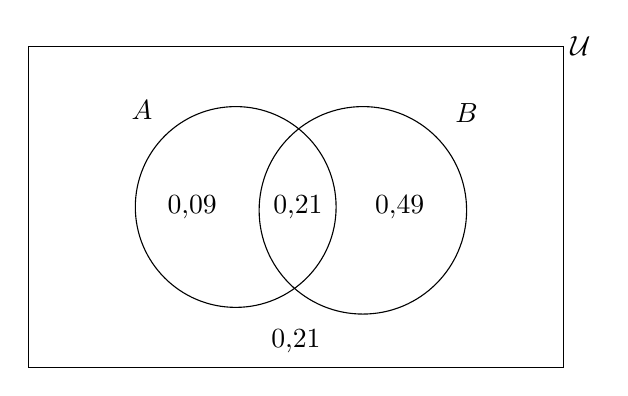
\begin{tikzpicture}[scale=0.85]
  \draw (-4,-2.4) rectangle (4,2.4);
  \draw (-0.9,0) circle (1.5);
  \draw (1.0,-0.05) circle (1.55);
  \node at (-2.3,1.45) {$A$};
  \node at (2.55,1.4) {$B$};
  \node at (4.25,2.4) {$\mathcal{U}$};
  \node at (-1.55,0) {0,09};
  \node at (0.03,0) {0,21};
  \node at (1.55,0) {0,49};
  \node at (0,-2.0) {0,21};
\end{tikzpicture}
\end{center}

\lienreponse{rep-ex1}
\end{frame}

\begin{frame}[t,label=ex6]{Exemple 6}

Il est possible que $A\perp B$, $A\perp C$ et $B\perp C$, sans que
$A,B,C$ soient (mutuellement) indépendants. Par exemple :

\begin{center}
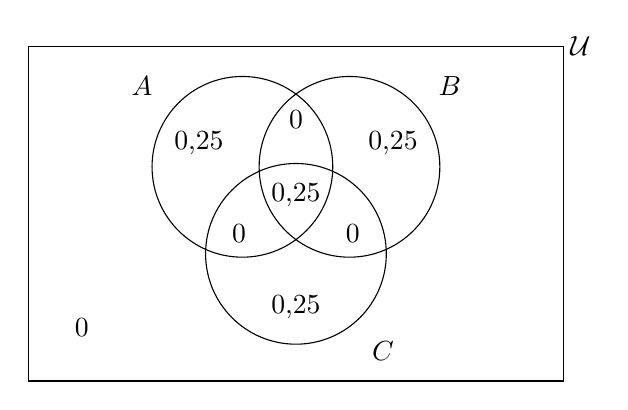
\begin{tikzpicture}[scale=0.85]
  \draw (-4,-2.6) rectangle (4,2.4);
  \draw (-0.8,0.6) circle (1.35);
  \draw (0.8,0.6) circle (1.35);
  \draw (0,-0.7) circle (1.35);
  \node at (-2.3,1.8) {$A$};
  \node at (2.3,1.8) {$B$};
  \node at (1.3,-2.15) {$C$};
  \node at (4.25,2.4) {$\mathcal{U}$};
  \node at (-1.45,0.95) {0,25};
  \node at (1.45,0.95) {0,25};
  \node at (0,-1.5) {0,25};
  \node at (0,0.17) {0,25};
  \node at (0,1.3) {0};
  \node at (-0.85,-0.4) {0};
  \node at (0.85,-0.4) {0};
  \node at (-3.2,-1.8) {0};
\end{tikzpicture}
\end{center}

\lienreponse{rep-ex1}
\end{frame}

\subsection{Loi des probabilités totales}

\begin{frame}[t]{Partitionner l'espace échantillonnal}

{\small Plusieurs calculs de probabilités deviennent plus simples si on
 les découpe en plusieurs morceaux.

 \begin{Boite}{Partition de l'espace échantillonnal}
  On dit que $B_1,B_2,\ldots,B_k$ forment une \alert{partition
  de $\mathcal{U}$} si et seulement si
  \begin{enumerate}
   \item ils sont mutuellement exclusifs, c'est-à-dire $B_i\cap B_j=\emptyset,\ \forall i\neq j$,\\

   \underline{et}
   \item leur union est $\mathcal{U}$ : $B_1\cup B_2\cup \cdots\cup B_k=\mathcal{U}$.
  \end{enumerate}
 \end{Boite}
}
\end{frame}

\begin{frame}[t]{Exemple d'une partition de $\mathcal{U}$}

\begin{center}
    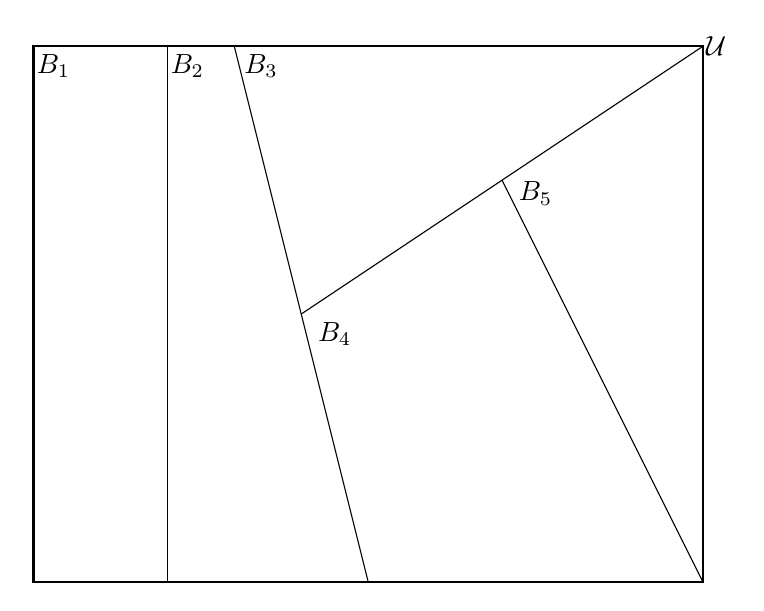
\begin{tikzpicture}[scale = 0.85]
  % L'espace échantillonnal
  \draw[thick] (-5,-4) rectangle (5,4);

  % Les frontières entre les morceaux
  \draw (-3,4) -- (-3,-4);
  \draw (-2,4) -- (0,-4);
  \draw (-1,0) -- (5,4);
  \draw (2,2) -- (5,-4);

  % Les étiquettes
  \node at (-4.7,3.7) {$B_1$};
  \node at (-2.7,3.7) {$B_2$};
  \node at (-1.6,3.7) {$B_3$};
  \node at (-0.5,-0.3) {$B_4$};
  \node at (2.5,1.8) {$B_5$};
  \node at (5.2, 4) {$\mathcal{U}$};

\end{tikzpicture}
\end{center}

\end{frame}

\begin{frame}[t]{Utilité de partitionner $\mathcal{U}$}
 \begin{Boite}{Lemme}
  Si $B_1,\ldots,B_k$ forment une partition de $\mathcal{U}$ et
  $A$ est un événement de $\mathcal{U}$, alors
  $$A=(A\cap B_1)\cup(A\cap B_2)\cup\cdots\cup(A\cap B_k).$$

  Puisque $(A\cap B_i)\cap(A\cap B_j)=\emptyset,\ \forall i\neq j$, on a
  \begin{align*}
  P(A)&=P(A\cap B_1)+P(A\cap B_2)+\cdots+P(A\cap B_k)\\
  \alert {P(A)} &\alert{=\sum_{i=1}^kP(A\cap B_i)}.
  \end{align*}
 \end{Boite}
\end{frame}

\begin{frame}[t]{Exemple d'une partition de $\mathcal{U}$ (suite)}

\begin{center}
    \begin{tikzpicture}[scale = 0.85]
  % L'espace échantillonnal
  \draw[thick] (-5,-4) rectangle (5,4);

  % Les frontières entre les morceaux
  \draw (-3,4) -- (-3,-4);
  \draw (-2,4) -- (0,-4);
  \draw (-1,0) -- (5,4);
  \draw (2,2) -- (5,-4);

  % L'événement A, à cheval sur plusieurs morceaux
  \draw[very thick, burntorange] (-0.5,0.3) ellipse (2.3 and 2.0);
  \node[burntorange] at (-0.5,1.6) {\bf A};

  % Les étiquettes
  \node at (-4.7,3.7) {$B_1$};
  \node at (-2.7,3.7) {$B_2$};
  \node at (-1.6,3.7) {$B_3$};
  \node at (-0.5,-0.3) {$B_4$};
  \node at (2.5,1.8) {$B_5$};
  \node at (5.2, 4) {$\mathcal{U}$};

\end{tikzpicture}
\end{center}
\end{frame}

\begin{frame}[t]{Cas d'une partition en deux événements}

\begin{columns}[T]
\begin{column}{0.5\textwidth}
\begin{tikzpicture}[scale = 0.7]
  \draw[thick] (-4,-3) rectangle (4,3);
  \draw (0,3) -- (0,-3);
  \draw[very thick, burntorange] (0,-0.2) ellipse (3 and 1.6);
  \node[burntorange] at (-1.6,-0.2) {\bf A};
  \node at (-3.5,2.6) {$B_1$};
  \node at (0.5,2.6) {$B_2$};
  \node at (4.4,3) {$\mathcal{U}$};
\end{tikzpicture}
\end{column}
\begin{column}{0.45\textwidth}
\end{column}
\end{columns}
\end{frame}

\begin{frame}[t]{Conditionner sur une partition pour trouver $P(A)$}
 \begin{thm}[Loi des probabilités totales]{}
  Soient $A$ un événement de $\mathcal{U}$ et $B_1,\ldots,B_k$ une partition
  de $\mathcal{U}$. Alors
  $$\begin{array}{llccccc}
P(A)&=& P(A\cap B_1) &+&\cdots&+&P(A\cap B_k)\\
&&&&&&\\
    &=&P(B_1)P(A|B_1)&+&\cdots&+&P(B_k)P(A|B_k)\\
&&&&&&\\
    &=&\multicolumn{5}{l}{\sum\limits_{i=1}^k P(B_i)P(A|B_i).}\\
\end{array}
$$
 \end{thm}


 \bigskip
 \underline{Cas particulier} : comme $B$ et $\overline{B}$ forment une partition
 de $\mathcal{U}$, on a $P(A)=P(A|B)P(B)+P(A|\overline{B})P(\overline{B})$.
\end{frame}
\begin{frame}[t,label=ex7]{Exemple 7}

{\small Je dors bien 75\,\% des nuits. Après une bonne nuit, mon code passe tous les
 tests du premier coup 90\,\% du temps. Après une mauvaise nuit, il les passe du
 premier coup seulement 20\,\% du temps.

\begin{enumerate}\itemsep 2cm
\item[a)] Quelle est la probabilité que j'aie mal dormi et que mon code ne passe pas
 tous les tests du premier coup?
\end{enumerate}

}
\lienreponse{rep-ex2}
\end{frame}
\begin{frame}[t]{Exemple 7 (suite)}

{\small
\begin{enumerate}\itemsep 2cm
\item[b)] Quelle est la probabilité que mon code passe tous les tests du premier coup?
\end{enumerate}


 \vspace{5 cm}

}
\lienreponse{rep-ex2}
\end{frame}

\begin{frame}[t]{Exemple 8}

{\footnotesize Dans un centre de données,
\begin{enumerate}[$\bullet$]
\item 50\,\% des disques durs viennent du fabricant A,
\item 30\,\% des disques durs viennent du fabricant B et
\item 20\,\% des disques durs viennent d'autres fabricants.
\end{enumerate}

On sait aussi que
\begin{enumerate}[$\circ$]
\item 90\,\% des disques du fabricant A fonctionnent plus de 5 ans sans panne,
\item cette proportion est de 80\,\% pour les disques du fabricant B
\item et de 70\,\% pour les disques des autres fabricants.
\end{enumerate}

\bigskip

}
\end{frame}

\begin{frame}[t]{Exemple 8 (suite)}
Tracez un diagramme en arbre et un diagramme de Venn qui représentent cette situation.
 \vspace{7cm}
\end{frame}


\begin{frame}[t,label=ex8]{Exemple 8 (suite)}
Quelle est la probabilité qu'un disque choisi au hasard dans ce centre de données fonctionne plus de 5 ans sans panne?

 \vspace{5.6cm}


\lienreponse{rep-ex2}
\end{frame}

\subsection{Théorème de Bayes}

\begin{frame}[t]{Quand l'information est donnée « à l'envers »...}
 Dans plusieurs problèmes, l'information est donnée sous la forme $P(A|B_i)$,
 mais on cherche plutôt $P(B_i|A)$.

 \begin{itemize}\itemsep 1cm
  \item Dans l'exemple de mon code (ex. 7), quelle est la probabilité que j'aie
  bien dormi, sachant que mon code a passé tous les tests du premier coup?
  \item Dans l'exemple des disques (ex. 8), si un disque est tombé en panne
  avant 5 ans, quelle est la probabilité qu'il vienne du fabricant B?
 \end{itemize}
\end{frame}

\begin{frame}
 \begin{thm}[Théorème de Bayes]{}
  Soient $A$ un événement de $\mathcal{U}$ et $B_1,\ldots,B_k$ une partition
  de $\mathcal{U}$. Alors
  $$P(B_j|A)=\frac{P(A|B_j)P(B_j)}{\sum_{i=1}^kP(A|B_i)P(B_i)},\ \ \forall j=1,\ldots,k.$$
 \end{thm}
C'est l'un des résultats les plus importants de la théorie des probabilités.

\end{frame}

\begin{frame}[t,label=ex7b]{Exemple 7 (suite)}

Aujourd'hui, mon code a passé tous les tests du premier coup (!).
\bigskip

Sachant cela, quelle est la probabilité que j'aie bien dormi?

\lienreponse{rep-ex2}
\end{frame}


\begin{frame}[t,label=quizbayes]

\centerline{\LARGE\bfseries\alert{QUIZ !}}
  Retournons à l'exemple 8. Un disque du centre de données est tombé en panne le mois passé,
  4 ans après son installation. Quelle est la probabilité qu'il vienne du fabricant B?
 \vspace{5cm}


\lienreponse{rep-quiz}
\end{frame}

\section{Permutations et combinaisons}

\begin{frame}[t]{Principe de multiplication}
 \begin{Boite}{Principe de multiplication}
  Si les ensembles $A_1,A_2,\ldots,A_k$ comptent respectivement $n_1,n_2,\ldots,n_k$
  éléments, il y a $n_1\times n_2\times\cdots\times n_k$ façons de choisir un élément
  dans chacun de ces ensembles.
 \end{Boite}

 \medskip
 Exemple : combien de codes postaux canadiens (de la forme A1A~1A1) peut-on former?
\end{frame}

\begin{frame}[t]{Permutations}
 \begin{defn}{}
  Une \alerter{permutation} est un arrangement \alerter{ordonné}
  d'objets \alerter{distincts}.
 \end{defn}

 \medskip

 \uncover<2->{
  \underline{Exemple} : \\
  Après un hackathon, il reste 3 pointes de pizza : pepperoni, végé et toute garnie.
  Deux personnes en veulent chacune une. De combien de façons
  différentes peut-on attribuer les pointes aux 2 personnes?
 }

\end{frame}

\begin{frame}{Permutations : formule générale}

 \begin{Boite}{Permutation}
  Le nombre de permutations de $n$ objets pris $r$
  à la fois est
  $$P_r^n=n(n-1)\cdots(n-r+1)=\frac{n!}{(n-r)!}.$$
 \end{Boite}

 \medskip

 \uncover<2->{
  Ce résultat découle du \alerter{principe de multiplication} : on a $n$
  choix d'objets pour la 1\textsuperscript{re} position, $n-1$ choix pour la
  2\textsuperscript{e}, ..., $n-r+1$ choix pour la $r$\textsuperscript{e}.
 }

 \medskip

 \uncover<3->{ [Rappel : $n!=n(n-1)(n-2)\cdots1$ et $0!=1!=1$, donc $P_n^n=n!$]}

 \medskip

 \uncover<4->{
  {\small Remarque : c'est un tirage \alerter{sans remise}, car un objet placé ne peut plus
  être choisi. Dans un tirage \alerter{avec remise}, on aurait $n$ choix à chaque position,
  donc $n^r$ arrangements.}
 }
\end{frame}

\begin{frame}[t,label=exdev]{Exemples}
\begin{itemize}
\item Dix développeurs sont disponibles pour prendre en charge quatre microservices
 distincts (un développeur par microservice). Combien y a-t-il de façons d'assigner
 les développeurs aux microservices?

\vspace{0.3in}

 \bigskip

 \uncover<2->{
  \item Pour ces 4 microservices, on doit aussi choisir 4 testeurs parmi
  12 testeurs disponibles (un testeur par microservice).\\ De combien de façons
  peut-on assigner les développeurs ET les testeurs aux 4 microservices?}

\vspace{0.15in}
 \end{itemize}
\lienreponse{rep-ex2}
\end{frame}

\subsection{Combinaisons}

\begin{frame}{Combinaisons}
 \begin{defn}{}
  Une \alerter{combinaison} est un arrangement
  \alerter{non ordonné} d'objets \alerter{distincts}.
 \end{defn}

 \medskip

 \uncover<2->{Exemple :\\
  Je dois choisir 2 de mes 3 meilleurs amis pour former une équipe avec moi
  au prochain hackathon. Combien d'options ai-je?
 }

 \medskip

 \uncover<3->{
  Soient $a,b,c$ mes trois meilleurs amis. \\
  Il y a $P^3_2=6$ permutations de ces 3 amis pris 2 à la fois... mais $(a,b)$
  et $(b,a)$ forment la même équipe!\\
  Il faut donc diviser $P^3_2$ par 2, ce qui donne 3 équipes possibles :
  $\{a,b\}$, $\{a,c\}$ et $\{b,c\}$.
 }
\end{frame}

\begin{frame}[t]{Combinaisons : formule générale}
 \begin{defn}{}
  Le nombre de combinaisons de $r$ objets choisis parmi $n$ est
  $${n\choose r}=C^n_r=\frac{n!}{r!(n-r)!}.$$
 \end{defn}

 \medskip

 \uncover<2->{
D'où vient cette formule?\\
\vspace{0.1 in}
  Soit $x$ le nombre de façons de choisir $r$ objets parmi $n$.
  Une permutation consiste à choisir d'abord $r$ objets parmi les $n$,
  puis à ordonner ces $r$ objets. Donc
  $$P^n_r=x\times P^r_r=x\, r! \quad\Rightarrow\quad x=\frac{P^n_r}{r!}=\frac{n!}{(n-r)!}\frac{1}{r!}=
  \frac{n!}{r!(n-r)!}.$$
 }
\end{frame}

\begin{frame}[t]{Exemples}
 \begin{itemize}
  \item<1->{\bf Lotto 6/49} : on tire au hasard, sans remise, 6 des 49 nombres de 1 à 49, et l'ordre dans
  lequel les 6 nombres sont tirés ne compte pas. Il y a donc
  \uncover<1->{
  $${49\choose6}=\frac{49!}{6!\,43!}=\frac{49\times48\times47\times46\times45\times44}{6!}=
  13~983~816$$
  combinaisons possibles. \\
  \vspace{0.1 in}
  Loto-Québec indique d'ailleurs sur son site web que la probabilité de gagner le gros lot est de $1/13~983~816$.
  \vspace{0.1in}

 {\small Note : on aurait aussi pu utiliser le principe de multiplication :
  49 choix pour le 1\textsuperscript{er} nombre, 48 pour le 2\textsuperscript{e}, ..., 44 pour le 6\textsuperscript{e}, puis diviser
  par $6!$, car chaque combinaison est comptée $6!$ fois.}}\\
 \end{itemize}
\end{frame}

\begin{frame}{Exemples (suite)}
 \begin{itemize}
  \item<1->{\bf Poker} : au poker, une main consiste en 5 cartes tirées d'un jeu de 52 cartes
  distinctes. Il y a donc
  $${52\choose5}=\frac{52!}{5!\,47!}=\frac{52\times51\times50\times49\times48}{5!}=
  2~598~960$$
  mains de poker distinctes.
 \end{itemize}
\end{frame}

\begin{frame}[t,label=expoker]{Exemples (suite)}


 \begin{itemize}
  \item{\bf Poker, paires} : quelle est la probabilité que la main obtenue soit une paire?\\
 \end{itemize}

   \vspace{0.1in}
\vspace{0.1in}


\lienreponse{rep-ex2}
\end{frame}

\begin{frame}[t,label=excomites]{Exemples (suite)}
 \begin{itemize}
  \item<1->{\bf Comités} : une association étudiante en informatique de 30 membres doit choisir 4 représentants.
  \begin{itemize} \itemsep1.3cm
  \item Combien de comités différents peut-on former?
  \item Et si le comité est formé d'un président, d'un vice-président, d'un trésorier
  et d'un secrétaire?
  \item Et si le comité est formé d'un président et de 3 autres membres?
  \end{itemize}
 \end{itemize}
\lienreponse{rep-ex2}
\end{frame}

\section{Compléments}

\begin{frame}[t]{Autres résultats découlant des axiomes}
 \begin{itemize}\itemsep6mm
  \item<1->{\bf Théorème 1.5} : généralisation du théorème 1.4 à $k$ événements :
     \\
$P\left(\bigcup\limits_{i=1}^kA_i\right)=\sum\limits_{i=1}^kP(A_i)
  -\sum\limits_{i=1}^k\sum\limits_{j=i+1}^kP(A_i\cap A_j)+\cdots+(-1)^{k-1}P\left(\bigcap\limits_{i=1}^kA_i\right)$

  \item<2->{\bf Théorème 1.6} : si $A\subset B$, alors $P(A)\le P(B)$.

  {\small \color{gray}{[$B=(\overline{A}\cap B)\cup A$, où $\overline{A}\cap B$ et $A$ sont mutuellement exclusifs...]}}
 \end{itemize}
\end{frame}

\begin{frame}{Théorème du binôme}

 \begin{thm}[Théorème du binôme]{}
  Soient deux nombres réels $x$ et $y$ et un entier $n\ge0$. Alors
  $$(x+y)^n=\sum_{r=0}^n{n\choose r}x^ry^{n-r}.$$
 \end{thm}

\end{frame}

\begin{frame}[t]{Identités utiles}
\vspace{0.5 in}
 \begin{itemize} \itemsep1cm
  \item ${n\choose r}={n\choose n-r}$
  \item ${n\choose r}={n-1\choose r-1}+{n-1\choose r}$
  \item $2^n=(1+1)^n=\sum_{r=0}^n {n\choose r}1^r1^{n-r}={n\choose0}+{n\choose1}
  +\cdots+{n\choose n}$
 \end{itemize}
\end{frame}



\section{Réponses des exemples}

\begin{frame}[t,label=rep-ex1]{Réponses des exemples (1/2)}
\footnotesize
\begin{itemize}
\item \retour{ex2s}{Exemple 2 (suite)} (aucun des deux problèmes) : $1-0{,}23=0{,}77$.
\item \retour{ex3}{Exemple 3} : (i) $0{,}45$~; (ii) manque d'information~; (iii) $0{,}45$~;
(iv) $0{,}30$~; (v) manque d'information~; (vi) $0{,}85$~; (vii) $P(L|S)=0{,}45/0{,}75=0{,}6$~;
(viii) $P(I|L)=0{,}35/0{,}55\approx0{,}636$.
\item \retour{ex4}{Exemple 4} : a) $0{,}10/0{,}70=1/7\approx0{,}143$~; b) $0{,}15/0{,}25=0{,}6$.
\item \retour{ex5}{Exemple 5} : $P(A)=0{,}30$, $P(B)=0{,}70$, $P(A)P(B)=0{,}21=P(A\cap B)$
$\Rightarrow$ $A$ et $B$ sont indépendants.
\item \retour{ex6}{Exemple 6} : $A,B,C$ sont indépendants deux à deux, mais
$P(A\cap B\cap C)=0{,}25\neq P(A)P(B)P(C)=0{,}125$ $\Rightarrow$ pas mutuellement
indépendants.
\end{itemize}
\end{frame}

\begin{frame}[t,label=rep-ex2]{Réponses des exemples (2/2)}
\footnotesize
\begin{itemize}
\item \retour{ex7}{Exemple 7} : a) $0{,}25\times0{,}80=0{,}20$~; b) $0{,}75\times0{,}90+0{,}25\times0{,}20=0{,}725$~;
(\hyperlink{ex7b}{suite, Bayes}) $P(\text{bien dormi}|\text{tests réussis})=\dfrac{0{,}90\times0{,}75}{0{,}725}=\dfrac{27}{29}\approx0{,}931$.
\item \retour{ex8}{Exemple 8} : $P(\text{fonctionne}>5\text{ ans})=0{,}5\times0{,}9+0{,}3\times0{,}8+0{,}2\times0{,}7=0{,}83$.
\item \retour{exdev}{Exemples} (développeurs) : $P^{10}_4=5~040$~; avec les testeurs : $5~040\times11~880=59~875~200$.
\item \retour{expoker}{Exemples} (poker, paires) : $1~098~240/2~598~960\approx0{,}423$ (42,3\,\%).
\item \retour{excomites}{Exemples} (comités) : $27~405$ comités~; $P^{30}_4=657~720$ (président, vice-président, trésorier,
secrétaire)~; $30\times{29\choose3}=109~620$ (président et 3 autres membres).
\end{itemize}
\end{frame}

\section{Réponses des quiz}

\begin{frame}[t,label=rep-quiz]{Réponses des quiz}
\footnotesize
\begin{itemize}
\item \retour{ex1}{Exemple 1} (mutuellement exclusifs) : $\mathcal{E}_1$ (dé) : oui, mutuellement exclusifs~;
$\mathcal{E}_4$ (temps de réponse) : non ($A\cap B=(150,175)\neq\emptyset$).
\item \retour{ex2}{Exemple 2} (téléphone) : a) $P(\overline{B})=1-0{,}20=0{,}80$~; b) $P(A\cap B)=
0{,}05+0{,}20-0{,}23=0{,}02$.
\item \retour{quizpab}{Quiz} ($P(B)>0$) : $P(A|B)=1$ si $B\subset A$~; $P(A|B)=P(A)/P(B)$ si
$A\subset B$~; $P(A|B)=0$ si $A$ et $B$ sont mutuellement exclusifs.
\item \retour{quizbayes}{Quiz} (disque en panne avant 5 ans) : $P(\text{fabricant }B|\text{panne avant 5 ans})=\dfrac{0{,}30\times0{,}20}{1-0{,}83}=\dfrac{6}{17}\approx0{,}353$.
\end{itemize}
\end{frame}

\begin{frame}{Bibliographie}
 	Ce document est rédigé avec Beamer ainsi qu'une classe .cls fournie par Jérôme Soucy. Les diapositives sont adaptées des diapositives créées par Anne-Sophie Charest
 pour le cours STT-1000 ainsi que celles créées par Thierry Duchesne et Emmanuelle Reny-Nolin pour le cours STT-1900. Les graphiques proviennent de ces deux sources.
 	\printbibliography
 	\vfill
 	\footnotesize Pour signaler une erreur dans ce document, veuillez écrire à l'adresse :~\href{mailto:julien.miron@mat.ulaval.ca}{julien.miron@mat.ulaval.ca}.
 \end{frame}

\end{document}
